\documentclass[tikz]{standalone}
\usetikzlibrary{arrows}

\begin{document}

  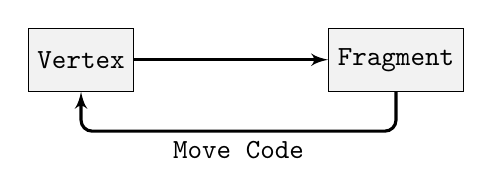
\begin{tikzpicture}[auto,font=\ttfamily,
    line/.style={draw, -latex', rounded corners, line width=0.4mm},
    shader/.style={draw, fill=gray!10,minimum size=8mm},
    ]
    % Place nodes
    \node [shader] (vs) {Vertex}; % keep
    \node [shader, right of=vs,xshift=30mm] (fs) {Fragment}; %

    % Draw edges
    \path [line] (vs) -- (fs);

    \draw [line] (fs.south) -- ++(0,-.5) -| node [near start] {Move Code} (vs.south);
  \end{tikzpicture}

\end{document}
